

\section{Introduction}

\label{sec:intro} One of the cornerstones of geometry is the problem
of packing circles and spheres into a container, e.g., a square or
a hypercube. It dates back to the 17th century when Kepler conjectured
his famous bound on the average density of any packing of spheres
in the three-dimensional Euclidean space~\cite{kepler2010six}. The problem has been investigated, for example, by Lagrange~\cite{chang2010simple}
who solved it in the setting of two dimensions, by Hales and Ferguson~\cite{hales2006formulation}
who proved Kepler's original conjecture, and by Viazovska~\cite{viazovska2017sphere}
who studied the problem in dimension $8$ and was awarded the Fields
medal in 2022 for her work.

A natural corresponding optimization question is the \emph{geometric
knapsack problem}, where we are given a set of $d$-dimensional objects
for some constant $d\in\mathbb{N}$, e.g., circles or \mbox{(hyper-)}spheres,
but possibly also other shapes (like squares, pentagons, hexagons,
etc. for the case of $d=2$) \agtwo{with} each of them having a given profit. The goal is to find the
subset of maximum total profit that can be packed non-overlappingly
into a given square or (hyper-)cube. \agtwo{In this work, we consider the translations of the objects but do not allow rotations.} 

Geometric knapsack is a natural mathematical problem and it is well-motivated
by practical applications in several areas, including radio tower
placement~\cite{szabo2007new}, origami design~\cite{lang1996computational},
cylinder pallet assembly~\cite{castillo2008solving,fraser1994integrated},
tree plantation~\cite{szabo2007new}, cutting industry~\cite{szabo2007new},
bundling tubes or cables~\cite{wang2002improved}, layout of control
panels~\cite{castillo2008solving}, or design of digital modulation
schemes~\cite{peikert1992packing}.

The problem is known to be \textsf{NP}-hard, already for $d=2$ and
if all input objects are \ari{axis-aligned} squares or disks \cite{demaine-Origami-NPHard,adamaszek2016hardness}.
This motivates designing approximation algorithms for it. For hypercubes
in any constant dimension $d$, there is a polynomial time $(1+\eps)$-approximation
algorithm is known for any constant $\eps>0$~\cite{Jansen0LS22}, i.e.,
a polynomial time approximation scheme (\textsf{PTAS}). Thus, this is the best
possible approximation guarantee, unless \textsf{P}=\textsf{NP}.

However, for other classes of (fat) objects, the best-known results
either have approximation ratios that are (far) from their respective lower
bounds or they require resource augmentation, i.e., an increase in the
size of the given knapsack. One intuitive reason for this is that
\ari{axis-aligned} squares and cubes can be stacked nicely without wasting space and
the resulting coordinates are well-behaved, while for more general
shapes this might not be the case, see \Cref{fig:corner}. %

\begin{figure}%[H]
	\centering 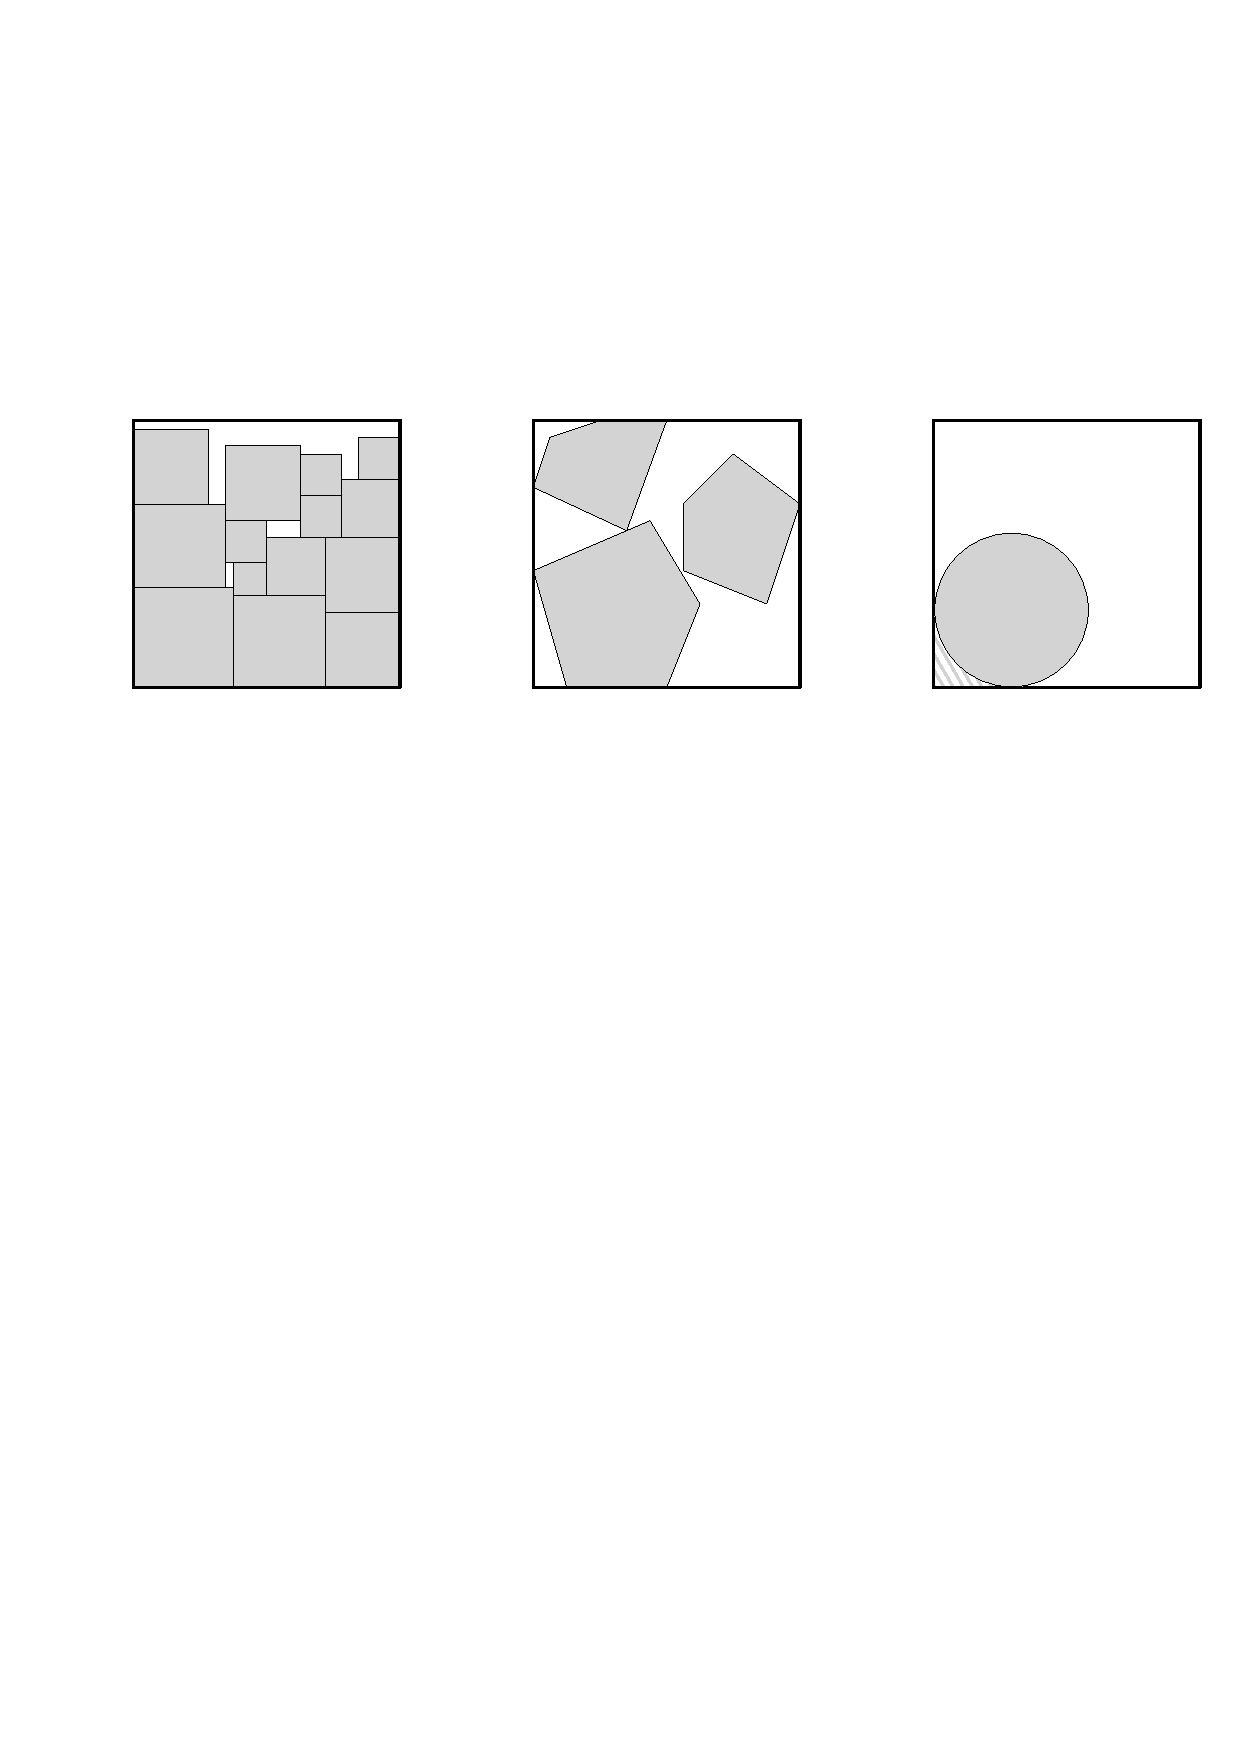
\includegraphics[width=1\textwidth]{Figures/intro}
	\caption{Left: The squares are stacked compactly inside the knapsack. Middle: The pentagons cannot
	be stacked as tightly inside the knapsack as the squares.
	Right: The space in the corner (striped area) cannot be covered by any large circle.}
	\label{fig:corner}
\end{figure}

For circles, the best known result is a $(3+\eps)$-approximation~\cite{Survey-Miyazawa}
but the best-known lower bound is only \textsf{NP}-hardness. 
\ari{Still, the membership in \textsf{NP} is wide open for the following question:
given a set of $n$ circles of $O(1)$ number of different sizes, decide whether they can be packed into a unit square.
 It is also open whether packing circles into a square knapsack is $\exists\mathbb{R}$-complete or not \cite{abrahamsen2020framework}. 
Even for $n$ unit circles,  we do not know the exact value of the smallest size squares that can pack them. 
See \cite{circP}  for the current status of
upper and lower bounds for $n \le 1000$. }

There
is a \textsf{PTAS} in any constant dimension $d$ for this case, but it requires
resource augmentation~\cite{MiyazawaWAOA}. For triangles, there
is a $O(1)$-approximation algorithm (assuming it is allowed to rotate
the triangles arbitrarily) whose precise approximation ratio is not
explicitly specified~\cite{MerinoW20}. Also for this case, it is
still possible that there is a \textsf{PTAS}.
On the other hand, there are settings of geometric knapsack
that do \emph{not} admit a \textsf{PTAS}, e.g., axis-parallel cuboids in three dimensions \cite{ChlebikC09}.


\ari{Furthermore, in practical applications (e.g., loading cargo into a truck or cutting pieces out of raw material like cloth or metal) the objects do not necessarily all have the same shape. For example, Bennell and Oliveira \cite{bennell2009tutorial}  consider a mix of different shapes of objects (their primary objects are circles, rectangles, regular polygons, and convex polygons).
However, the previous papers in the theoretical literature for geometric knapsacks mostly assume that all input objects are of the same type, e.g., only squares, only circles, or only rectangles, etc. Thus, from a theoretical point of view, it is interesting to see how the problem behaves when the input objects might be of different types.}

This raises the following natural question that we study in this paper:
\begin{center}
\emph{What are the best approximation ratios we can achieve for the
geometric knapsack problem, depending on the type of the input objects?
For which type of objects does a \textsf{PTAS} exist?}
\par\end{center}

\subsection{Our contribution}

In this paper, we present a polynomial time $(1+\eps)$-approximation algorithm for the geometric knapsack problem for packing  
$d$-dimensional spheres into $d$-dimensional hypercube knapsack, for any constant dimension $d \ge 2$. For spheres,
there is a complication that possibly any (near-)optimal
\agtwo{packing} for a given instance requires irrational coordinates. Therefore,
our output consists of a set of spheres that can be packed non-overlappingly
inside the given knapsack and whose profit is at least \ag{$(1+\eps)^{-1}w\mathrm{(OPT)}$,
where $w\mathrm{(OPT)}$ denotes the profit of the optimal solution $\mathrm{OPT}$}.
Moreover, for all but at most $O_{\varepsilon}(1)$ spheres, our algorithm
outputs the precise (rational) coordinates of the packing. \footnote{The notation $O_{\eps}(f(n))$ means that the implicit constant hidden in big-$O$ notation can depend on $\eps$.}
For the other $O_{\varepsilon}(1)$
spheres it outputs them up to an exponentially small error in each
dimension. We remark that there are related packing problems for which
it is known that irrational coordinates are sometimes necessary and
that computing them is $\exists\mathbb{R}$-complete (and hence possibly
even harder than \textsf{NP}-hardness) \cite{abrahamsen2020framework}.
On the other hand, if we knew that there always exists a $(1+\eps)$-approximate
solution in which all coordinates are rational with only a polynomial
number of bits, our algorithm would find such coordinates in polynomial
time. We stress that our returned set of spheres is always guaranteed
to fit into the given knapsack with appropriate (possibly irrational)
coordinates but \emph{without} resource augmentation.

Our second result is a polynomial time $(1+\eps)$-approximation
\agtwo{algorithm} for the geometric knapsack problem for wide classes of
convex geometric polygons. We give a \textsf{PTAS} for a class of
fat convex polygons which generalizes pentagons, hexagons, and regular
$k$-gons for constant $k>4$ (see \Cref{fig:regular-obj-packing}). Formally, we require
for each polygon that the angle between any two adjacent edges is
at least $\pi/2+\delta$ for some constant $\delta>0$ and that each
polygon has a constant number of edges with similar lengths (up to
a constant factor). Note that in contrast to many prior results, we
allow each input object to have a different shape, e.g., with a different
number of edges, different angles formed by them, and a different
orientation. Also, the polygons may differ arbitrarily in size.

\begin{figure}%[H]
	\centering 
\includegraphics[width=0.5\textwidth]{Figures/regular-obj-packing}
	% Scale image to the width of the text
	\caption{Packing of fat convex polygons in a knapsack}
	\label{fig:regular-obj-packing}
\end{figure}


If each input object is sufficiently small compared to the knapsack,
% i.e., at most
% a $\Theta(\epsilon)$-ratio of the size of the knapsack,
we obtain
even a polynomial time $(1+\eps)$-approximation for \emph{arbitrary}
fat convex \ari{objects} in any constant dimension $d$. We remark that for other packing problems like
one-dimensional \textsc{Knapsack} or \textsc{Bin Packing}, near-optimal
solutions can easily be achieved via greedy algorithms if the input
objects are sufficiently small. 
\ari{Even for sufficiently small $d$-dimensional axis-aligned hypercuboids, it is known that simple algorithms like NFDH \cite{NFDH, bansal2006bin} have negligible wasted space. 
However, for other geometric objects this
is much harder since we might not be able to place the input objects
compactly without wasting space. 
For example, classical result by Thue \cite{chang2010simple} showed that one can pack at most 
$\frac{\pi}{2 \sqrt{3}} \approx 0.9069$ fraction of the total area, even in the case of packing of unit circles.  
Furthermore, for circles and other similar convex objects, irrational coordinates may arise in the packing and the optimal solution may use a very complicated packing to minimize the wasted space.}

\subsection{Our techniques}
Now, we discuss the techniques of our results, starting with our \textsf{PTAS}
for spheres. To compute our packing, we first enumerate all the large
spheres in the optimal solution, i.e., the spheres whose radius is
at least a constant fraction of the side length of the knapsack. Also,
we guess their placement up to a polynomially small error, which yields
a small range of possible placements for each of them. Note that we
cannot guess these coordinates precisely, since we cannot even exclude
that they are irrational. However, we guarantee that such coordinates
\emph{exist}, by solving a system of polynomial equations \emph{exactly
}in polynomial time.
% \textcolor{red}
{Polynomial inequalities (semi-algebraic sets) have previously been applied in the context of circle packing problems \cite{szabo2005global}. 
For instance, Miyazawa et al. \cite{MiyazawaPSSW16} employed polynomial inequalities for the circle bin packing problem. 
We remark that we introduce the new idea of first guessing the coordinates up to a small error, thanks to which we know that we placed the spheres almost at their correct coordinates.}

Next, we want to place small spheres into the remaining part of the
knapsack. Unfortunately, we do not know precisely which part of the
knapsack is available for them since we do not know the precise coordinates
of the large spheres. Thus, there is some area of the knapsack that
is \emph{maybe} used by the large spheres in our packing; however, potentially, the
optimal solution uses it for placing small spheres. Our key insight
is that this area is small compared to the area that is for
sure \emph{not} used by large spheres in the optimal solution. Using the
fact that objects are spheres, we show that some area in each corner
of the knapsack cannot be covered by any large sphere in \emph{any}
solution and whose size is at least a constant fraction of the knapsack
(see the bottom-left empty corner in \Cref{fig:corner}). We use this area to compensate for the fact that we
do not know the precise coordinates of our large spheres and we waste
space because of this.


When we select and pack the small spheres, we define a constant number
of (small) identical knapsacks that fit into the given knapsack together
with the large spheres and into which we place our small spheres.
For the remaining task of placing the small spheres, we argue that it is sufficient to have an algorithm
that uses resource augmentation, i.e., that increases the size of
each knapsack by a factor of $1+\eps$ (in each dimension).
Thus, on a high level, we reduce the problem of packing arbitrary spheres
into \emph{one} knapsack to the problem of packing small spheres into
a \emph{constant number} of knapsacks \emph{with resource augmentation}.


% \textcolor{red}
{In order to solve the remaining problem, we use a hierarchical decomposition,
similar to, e.g., \cite{ErlebachJS05, JansenS08, MiyazawaPSSW16, MiyazawaWAOA}. In particular, Miyazawa et al. \cite{MiyazawaPSSW16} employ such a decomposition for the circle bin packing problem and argue that it is possible to first pack the relatively large circles, partition the remaining space in the bins into smaller sub-bins for smaller circles, and continue recursively.
Furthermore, for the circle knapsack problem
Miyazawa et al.~\cite{MiyazawaWAOA} introduced a sophisticated strategy based on a hierarchical decomposition that uses a combination of two configuration-based integer programs (IP). 
In this work, we use a rather bottom-up approach and provide a dynamic program based solution, which is arguably simpler than the corresponding algorithm in \cite{MiyazawaWAOA} and we also show that our subroutine works for arbitrary convex fat objects which is a larger class of objects.
Intuitively, in the structured packing the grid cells are
partitioned such that each placed object $P$ is contained in a constant number of grid cells
whose size is comparable to $P$. Importantly, these grid cells are used \emph{exclusively} by $P$
and not by any other placed object (not even partially). 
Our DP has a subproblem
for each combination of a level (corresponding to a size range of the input objects) and a number of
available grid cells corresponding to this level.
Given such a subproblem, it suffices to enumerate a polynomial number of possibilities for selecting and placing
objects of this level, which reduces the given subproblem
to a subproblem corresponding to the next level. This DP might have applications in other related packing problems. 


In our algorithm for fat convex polygons (with the properties described
above), we extend our algorithm for spheres as follows. For the
guessed large polygons, we compute their coordinates \emph{exactly
}in polynomial time. Here, we use the (known) fact that there exists
a placement for them that corresponds to an extreme point solution
of a suitable linear program, which has rational coordinates. Then,
intuitively we use the condition for the polygons' angles to ensure
that the large objects leave a certain area of the knapsack empty.
We use this empty area in a similar way as in the setting of circles.
Again, we place the small objects into a constant number of knapsacks
under resource augmentation, using our new subroutine described above.


If all input objects are sufficiently small compared to the size of the knapsack (formally, we assume that each of them
fits in a smaller knapsack with side length $\Theta(\eps)$)
there are no large objects and, hence,
we can omit the step of enumerating them. In particular, we do not
need the conditions of the polygons' edges anymore.
Since the input objects are so small,
we can show that by losing a factor of $1+\eps$ in the approximation ratio,
we may pretend that we have resource augmentation available.
Hence, we can directly call our subroutine for small objects under resource augmentation.

We leave it as an open question to determine whether irrational coordinates
are sometimes necessary for $(1+\eps)$-approximate 
solutions for geometric knapsack for spheres, i.e., if values $\eps>0$ exist for which this is the case.
If yes, it would be
interesting to determine the best possible approximation ratio one
can achieve with rational coordinates only. Note that this question
is related to the well-studied problem of determining the size of
the smallest knapsack needed to pack a given number of unit circles.
For that problem, it is known that for some number of unit circles
the smallest knapsack has irrational edge lengths~\cite{friedman-cirinsqu}.
On the other hand, recall that if rational coordinates with a polynomial number of bits
always suffice, our algorithm for spheres can compute the coordinates
of \emph{all} returned spheres of our $(1+\eps)$-approximation algorithm
\emph{exactly}.

\subsection{Other related work}
{Two related problems are the geometric bin packing and geometric strip packing problems.
In geometric bin packing, we want to place a given set of geometric objects non-overlappingly into the smallest possible number
of unit-size bins. 
In the strip packing problem, the objective is to pack a set of geometric objects non-overlappingly  into a strip of unit
width and minimum height.
Miyazawa, Pedrosa, Schouery, Sviridenko, and Wakabayashi \cite{MiyazawaPSSW16} gave an \textsf{APTAS} for the circle bin packing problem with resource augmentation, and
an \textsf{APTAS} for the circle strip packing problem. Their framework extends to a wide range of geometric packing problems, e.g., with ellipses, regular polygons, $d$-dimensional spheres under $L_p$-norm, etc.
They also posed the question of whether it is always possible to obtain a rational solution to the problem of packing a set of circles with rational radii in a non-augmented bin of rational coordinates. 
Lintzmayer, Miyazawa, and Xavier~\cite{lintzmayer2018two} used the structure of
solutions presented by \cite{MiyazawaPSSW16}, in combination with new ideas, to obtain a \textsf{PTAS} for the circle knapsack problem
under resource
augmentation in one dimension, assuming that the profit of each circle
equals its area. 
This was recently improved by Chagas, Dell\textquoteright Arriva, and Miyazawa~\cite{MiyazawaWAOA} to the earlier mentioned \textsf{PTAS} under resource augmentation in one dimension for spheres with arbitrary profits in any constant
dimension $d$. 
In addition, there have been many attempts to develop heuristics and
other optimization methods on circle packing, see e.g.,~\cite{szabo2007new,hifi2009literature,lubachevsky1997curved}.}

Recently, independently and parallel to our work, Chagas, Dell\textquoteright Arriva, and Miyazawa~\cite{ChagasNew} have also obtained similar results as the results we present in this paper. They have given a \textsf{PTAS} for the hypersphere multiple knapsack problem. Additionally, they can handle common constraints such as conflict constraints (some pairs of items cannot be packed together), multiple-choice constraints (given a subset of items, at most one of them can be packed), and capacity constraints (items additionally have associated weights, and the sum of weights of the packed items cannot exceed the weight capacity of the knapsack). Moreover, they extended the results to a wide range of convex fat objects, such as, ellipsoids, rhombi, and hyperspheres under $L_p$-norms. 
Furthermore, they provided a resource augmentation scheme for fat objects where rotations are allowed. Finally, they 
show that their framework can be extended to other problems, such as 
the cutting stock problem, the minimum-size bin packing problem, and the multiple strip packing problem.}



Geometric packing problems are also well-studied for rectangular objects. 
For geometric knapsack for axis-parallel rectangles (i.e., when $d=2$),
the best known polynomial time algorithm has an approximation ratio of $17/9+\eps$~\cite{galvez2017approximating}. 
There is a pseudo-polynomial time algorithm with a ratio of $4/3+\eps$
\cite{galvez2021improved} and a pseudo-polynomial time approximation scheme if we require guillotine-separable packing \cite{KhanMSW21}. If it is allowed to rotate the rectangles
by 90 degrees, there is also a polynomial time $(1.5+\eps)$-approximation
algorithm known~\cite{galvez2017approximating}. Moreover, the problem
admits a \textsf{QPTAS} if the input data are quasi-polynomially bounded integers~\cite{adamaszek2014quasi}.
For the settings of geometric bin packing with squares or (hyper-)cubes \cite{bansal2006bin} or skewed rectangles \cite{KhanS23},  
the problem \agtwo{admits} an asymptotic \textsf{PTAS}. In the
case of general rectangles, the best-known result is an asymptotic $1.405$-approximation~\cite{bansal2014improved}
but an asymptotic \textsf{PTAS} cannot exist unless $\mathsf{P=NP}$~\cite{ChlebikC09}.
Maximum independent set in geometric intersection graphs \cite{ChanH12, Mitchell21, GalvezKMMPW22} is another well-studied related problem. 

In a recent paper, Abrahamsen, Miltzow, and Seiferth~\cite{abrahamsen2020framework}
developed a framework to show that for many combinations of allowed
pieces, containers, and motions, the resulting packing problem is
$\exists\mathbb{R}$-complete. For example, they showed that it is
$\exists\mathbb{R}$-complete problem to decide if a set of convex
polygons with at most seven corners each can be packed into a square
if arbitrary rotations are allowed. 
However, it is not known if the setting of packing circles into a
square knapsack is $\exists\mathbb{R}$-complete.

There is also a large body of work on questions about the optimal packings of unit circles into unit squares or equilateral triangles.
We refer to \cite{fekete2023packing, fodor2003densest, goldberg1971packing, hifi2009literature} for an overview. 


\subsection{Organization of this paper}
In Section \ref{sec:ptas-ra}, we discuss the \textsf{PTAS} when the input items are sufficiently small fat convex objects. In Section \ref{sec:spheres}, we give our \agtwo{algorithm} for spheres.
In Section \ref{sec:polygon}, we consider the case of convex polygons.  Finally, in Section \ref{sec:conc} we end with conclusions. 
Some proofs have been presented in the appendix. 
The corresponding lemmas and theorems are marked with~$(\star)$.
%Please see the full version of the paper for the complete proofs. 


